
\section{Numerical summaries}

\R\ includes a number of commands to numerically summarize variables.
These include the capability of calculating the mean, standard deviation,
variance, median, five number summary, interquartile range (IQR) as well as arbitrary quantiles.  We will
illustrate these using the CESD (Center for Epidemiologic Studies--Depression)
measure of depressive symptoms (which takes on values between 0 and 60, with higher
scores indicating more depressive symptoms).  

To improve the legibility of output,
we will also set the default number of digits to display to a more reasonable
level (see \function{?options} for more configuration possibilities).

\myindex{HELPrct dataset}%
\Rindex{options()}%
\Rindex{require()}%
\Rindex{mosaic package}%
\begin{knitrout}
\definecolor{shadecolor}{rgb}{0.969, 0.969, 0.969}\color{fgcolor}\begin{kframe}
\begin{alltt}
\hlkwd{require}\hlstd{(mosaic)}
\end{alltt}


{\ttfamily\noindent\itshape\color{messagecolor}{\#\# Loading required package: mosaic}}

{\ttfamily\noindent\itshape\color{messagecolor}{\#\# Loading required package: dplyr}}

{\ttfamily\noindent\itshape\color{messagecolor}{\#\# \\\#\# Attaching package: 'dplyr'}}

{\ttfamily\noindent\itshape\color{messagecolor}{\#\# The following objects are masked from 'package:stats':\\\#\# \\\#\#\ \ \ \  filter, lag}}

{\ttfamily\noindent\itshape\color{messagecolor}{\#\# The following objects are masked from 'package:base':\\\#\# \\\#\#\ \ \ \  intersect, setdiff, setequal, union}}

{\ttfamily\noindent\itshape\color{messagecolor}{\#\# Loading required package: lattice}}

{\ttfamily\noindent\itshape\color{messagecolor}{\#\# Loading required package: ggformula}}

{\ttfamily\noindent\itshape\color{messagecolor}{\#\# Loading required package: ggplot2}}

{\ttfamily\noindent\itshape\color{messagecolor}{\#\# \\\#\# New to ggformula?\ \ Try the tutorials: \\\#\# 	learnr::run\_tutorial("{}introduction"{}, package = "{}ggformula"{})\\\#\# 	learnr::run\_tutorial("{}refining"{}, package = "{}ggformula"{})}}

{\ttfamily\noindent\itshape\color{messagecolor}{\#\# Loading required package: mosaicData}}

{\ttfamily\noindent\itshape\color{messagecolor}{\#\# Loading required package: Matrix}}

{\ttfamily\noindent\itshape\color{messagecolor}{\#\# \\\#\# The 'mosaic' package masks several functions from core packages in order to add \\\#\# additional features.\ \ The original behavior of these functions should not be affected by this.\\\#\# \\\#\# Note: If you use the Matrix package, be sure to load it BEFORE loading mosaic.}}

{\ttfamily\noindent\itshape\color{messagecolor}{\#\# \\\#\# Attaching package: 'mosaic'}}

{\ttfamily\noindent\itshape\color{messagecolor}{\#\# The following object is masked from 'package:Matrix':\\\#\# \\\#\#\ \ \ \  mean}}

{\ttfamily\noindent\itshape\color{messagecolor}{\#\# The following objects are masked from 'package:dplyr':\\\#\# \\\#\#\ \ \ \  count, do, tally}}

{\ttfamily\noindent\itshape\color{messagecolor}{\#\# The following objects are masked from 'package:stats':\\\#\# \\\#\#\ \ \ \  binom.test, cor, cor.test, cov, fivenum, IQR, median,\\\#\#\ \ \ \  prop.test, quantile, sd, t.test, var}}

{\ttfamily\noindent\itshape\color{messagecolor}{\#\# The following objects are masked from 'package:base':\\\#\# \\\#\#\ \ \ \  max, mean, min, prod, range, sample, sum}}\begin{alltt}
\hlkwd{require}\hlstd{(mosaicData)}
\hlkwd{options}\hlstd{(}\hlkwc{digits}\hlstd{=}\hlnum{4}\hlstd{)}
\hlkwd{mean}\hlstd{(}\hlopt{~} \hlstd{cesd,} \hlkwc{data}\hlstd{=HELPrct)}
\end{alltt}
\begin{verbatim}
## [1] 32.85
\end{verbatim}
\end{kframe}
\end{knitrout}

\myindex{Start Teaching with R@\emph{Start Teaching with R}}%
\myindex{Teaching with R@\emph{Teaching with R}}%
\myindex{Start Modeling with R@\emph{Start Modeling with R}}%
\myindex{Modeling with R@\emph{Modeling with R}}%
Note that the \function{mean()} function in the \pkg{mosaic} package supports a formula interface common to \pkg{lattice} graphics and linear models (e.g., \function{lm()}).  The \pkg{mosaic} package provides many other functions that use the same notation, which we will be using throughout this document.  
\DiggingDeeper[-3cm]{If you have not seen the formula notation before, the companion book, \emph{Start Teaching with R} provides a detailed presentation.  \emph{Start Modeling with R}, another companion book, details the relationship between the process of modeling and the formula notation. }

\Rindex{with()}%
\Rindex{mean()}%
The same output could be created using the following commands (though we will use the MOSAIC versions when available).
\begin{knitrout}
\definecolor{shadecolor}{rgb}{0.969, 0.969, 0.969}\color{fgcolor}\begin{kframe}
\begin{alltt}
\hlkwd{with}\hlstd{(HELPrct,} \hlkwd{mean}\hlstd{(cesd))}
\end{alltt}
\begin{verbatim}
## [1] 32.85
\end{verbatim}
\begin{alltt}
\hlkwd{mean}\hlstd{(HELPrct}\hlopt{$}\hlstd{cesd)}
\end{alltt}
\begin{verbatim}
## [1] 32.85
\end{verbatim}
\end{kframe}
\end{knitrout}
\Rindex{sd()}%
\Rindex{var()}%
Similar functionality exists for other summary statistics.
\begin{knitrout}
\definecolor{shadecolor}{rgb}{0.969, 0.969, 0.969}\color{fgcolor}\begin{kframe}
\begin{alltt}
\hlkwd{sd}\hlstd{(}\hlopt{~} \hlstd{cesd,} \hlkwc{data}\hlstd{=HELPrct)}
\end{alltt}
\begin{verbatim}
## [1] 12.51
\end{verbatim}
\end{kframe}
\end{knitrout}
\begin{knitrout}
\definecolor{shadecolor}{rgb}{0.969, 0.969, 0.969}\color{fgcolor}\begin{kframe}
\begin{alltt}
\hlkwd{sd}\hlstd{(}\hlopt{~} \hlstd{cesd,} \hlkwc{data}\hlstd{=HELPrct)}\hlopt{^}\hlnum{2}
\end{alltt}
\begin{verbatim}
## [1] 156.6
\end{verbatim}
\begin{alltt}
\hlkwd{var}\hlstd{(}\hlopt{~} \hlstd{cesd,} \hlkwc{data}\hlstd{=HELPrct)}
\end{alltt}
\begin{verbatim}
## [1] 156.6
\end{verbatim}
\end{kframe}
\end{knitrout}

It is also straightforward to calculate quantiles of the distribution.

\myindex{quantiles}%
\Rindex{median()}%
\begin{knitrout}
\definecolor{shadecolor}{rgb}{0.969, 0.969, 0.969}\color{fgcolor}\begin{kframe}
\begin{alltt}
\hlkwd{median}\hlstd{(}\hlopt{~} \hlstd{cesd,} \hlkwc{data}\hlstd{=HELPrct)}
\end{alltt}
\begin{verbatim}
## [1] 34
\end{verbatim}
\end{kframe}
\end{knitrout}

By default, the \function{quantile()} function displays the quartiles, but can be given a vector of quantiles to display.  
\Rindex{quantile()}%
\Caution{Not all commands have been upgraded to
support the formula interface. For these functions, variables within dataframes must be accessed using \function{with()} or the \$ operator.}
\begin{knitrout}
\definecolor{shadecolor}{rgb}{0.969, 0.969, 0.969}\color{fgcolor}\begin{kframe}
\begin{alltt}
\hlkwd{with}\hlstd{(HELPrct,} \hlkwd{quantile}\hlstd{(cesd))}
\end{alltt}
\begin{verbatim}
##   0%  25%  50%  75% 100% 
##    1   25   34   41   60
\end{verbatim}
\begin{alltt}
\hlkwd{with}\hlstd{(HELPrct,} \hlkwd{quantile}\hlstd{(cesd,} \hlkwd{c}\hlstd{(}\hlnum{.025}\hlstd{,} \hlnum{.975}\hlstd{)))}
\end{alltt}
\begin{verbatim}
##  2.5% 97.5% 
##   6.3  55.0
\end{verbatim}
\end{kframe}
\end{knitrout}

\hfill

\Rindex{favstats()}%
Finally, the \function{favstats()} function in the \pkg{mosaic} package provides a concise summary of  many useful statistics.
\begin{knitrout}
\definecolor{shadecolor}{rgb}{0.969, 0.969, 0.969}\color{fgcolor}\begin{kframe}
\begin{alltt}
\hlkwd{favstats}\hlstd{(}\hlopt{~} \hlstd{cesd,} \hlkwc{data}\hlstd{=HELPrct)}
\end{alltt}
\begin{verbatim}
##  min Q1 median Q3 max  mean    sd   n missing
##    1 25     34 41  60 32.85 12.51 453       0
\end{verbatim}
\end{kframe}
\end{knitrout}

\section{Graphical summaries}
The \function{histogram()} function is used to create a histogram. Here we use the formula interface (as discussed in the \emph{Start Modeling with R} book) to specify that we want a histogram of the CESD scores.

\Rindex{histogram()}%
\vspace{-4mm}
\begin{center}
\begin{knitrout}
\definecolor{shadecolor}{rgb}{0.969, 0.969, 0.969}\color{fgcolor}\begin{kframe}
\begin{alltt}
\hlkwd{gf_histogram}\hlstd{(}\hlopt{~} \hlstd{cesd,} \hlkwc{data} \hlstd{= HELPrct,} \hlkwc{binwidth} \hlstd{=} \hlnum{2.4}\hlstd{)} \hlopt
  \hlkwd{gf_labs}\hlstd{(}\hlkwc{title} \hlstd{=} \hlstr{""}\hlstd{)}
\end{alltt}
\end{kframe}
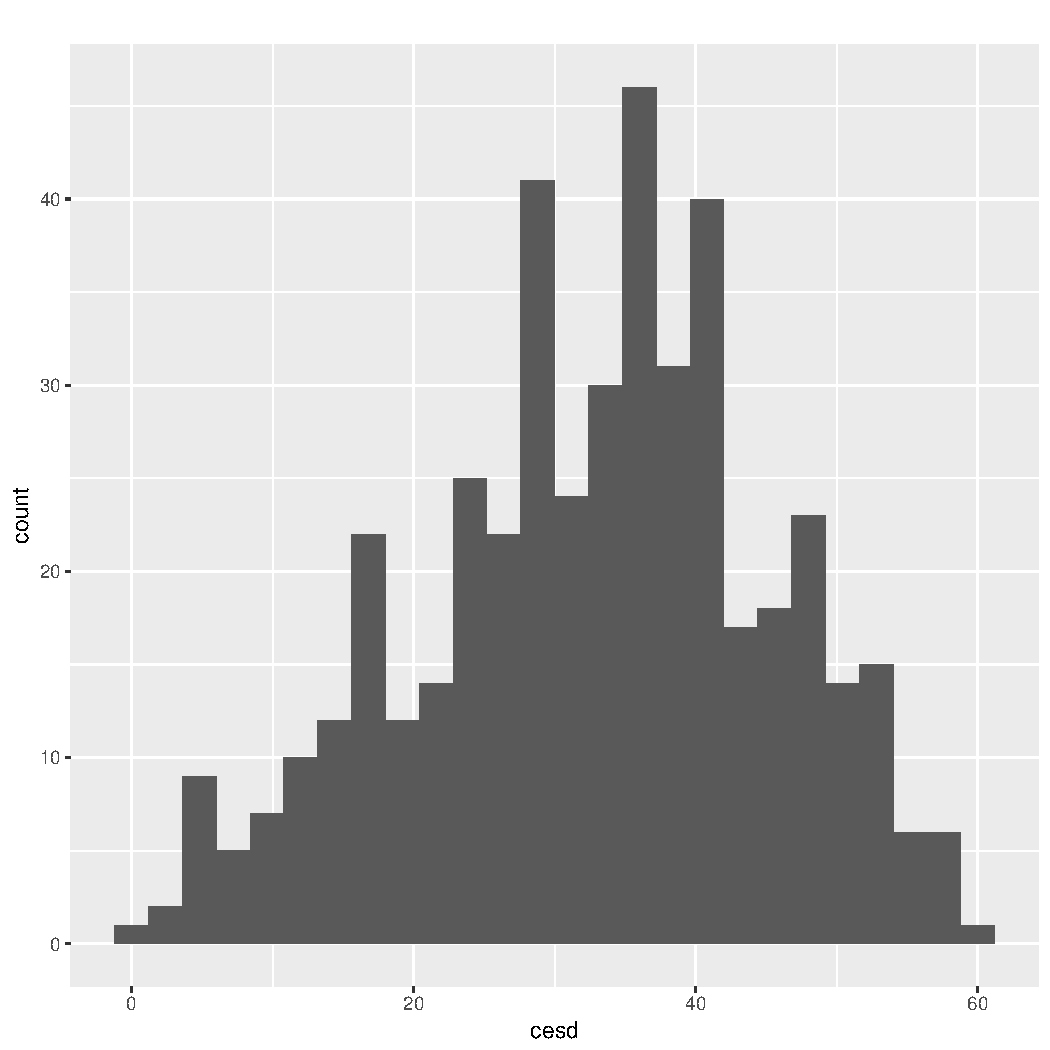
\includegraphics[width=\maxwidth]{figure/cesd-hist-1} 

\end{knitrout}
\end{center}

We can use the \function{width} and \function{center} options to control the location of the bins.

\begin{center}
\begin{knitrout}
\definecolor{shadecolor}{rgb}{0.969, 0.969, 0.969}\color{fgcolor}\begin{kframe}
\begin{alltt}
\hlkwd{histogram}\hlstd{(}\hlopt{~} \hlstd{cesd,} \hlkwc{width}\hlstd{=}\hlnum{5}\hlstd{,} \hlkwc{center}\hlstd{=}\hlnum{2.5}\hlstd{,} \hlkwc{data}\hlstd{=HELPrct)}
\end{alltt}
\end{kframe}
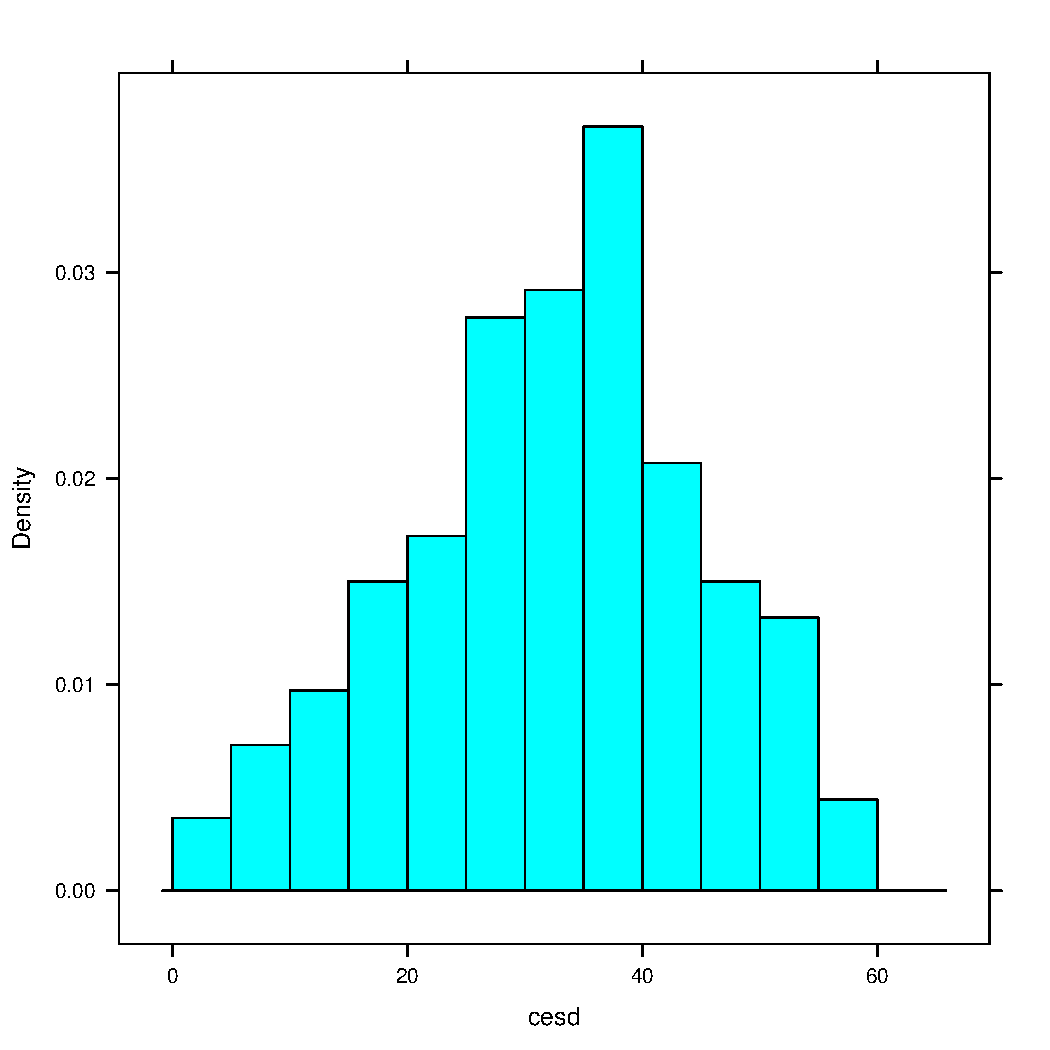
\includegraphics[width=\maxwidth]{figure/cesd-hist2-1} 

\end{knitrout}
\end{center}


\Rindex{tally()}%
\Rindex{format option}%
In the \variable{HELPrct} dataset, approximately one quarter of the subjects are female.  
\begin{knitrout}
\definecolor{shadecolor}{rgb}{0.969, 0.969, 0.969}\color{fgcolor}\begin{kframe}
\begin{alltt}
\hlkwd{tally}\hlstd{(}\hlopt{~} \hlstd{sex,} \hlkwc{data}\hlstd{=HELPrct)}
\end{alltt}
\begin{verbatim}
## sex
## female   male 
##    107    346
\end{verbatim}
\begin{alltt}
\hlkwd{tally}\hlstd{(}\hlopt{~} \hlstd{sex,} \hlkwc{format}\hlstd{=}\hlstr{"percent"}\hlstd{,} \hlkwc{data}\hlstd{=HELPrct)}
\end{alltt}
\begin{verbatim}
## sex
## female   male 
##  23.62  76.38
\end{verbatim}
\end{kframe}
\end{knitrout}

It is straightforward to restrict our attention to just the female subjects.
If we are going to do many things with a subset of our data, it may be easiest
to make a new dataframe containing only the cases we are interested in.
The \function{filter()} function in the \pkg{dplyr} package can be used to generate a new dataframe containing
just the women or just the men  (see also section \ref{sec:subsets}).  Once this is created, the
the \function{stem()} function is used to create a stem and leaf plot.
\Caution{Note that the tests for equality use \emph{two} equal signs}
\Rindex{stem()}%
\Rindex{filter()}%
\Rindex{dplyr package}%
\begin{knitrout}
\definecolor{shadecolor}{rgb}{0.969, 0.969, 0.969}\color{fgcolor}\begin{kframe}
\begin{alltt}
\hlstd{female} \hlkwb{<-} \hlkwd{filter}\hlstd{(HELPrct, sex}\hlopt{==}\hlstr{'female'}\hlstd{)}
\hlstd{male} \hlkwb{<-} \hlkwd{filter}\hlstd{(HELPrct, sex}\hlopt{==}\hlstr{'male'}\hlstd{)}
\hlkwd{with}\hlstd{(female,} \hlkwd{stem}\hlstd{(cesd))}
\end{alltt}
\begin{verbatim}
## 
##   The decimal point is 1 digit(s) to the right of the |
## 
##   0 | 3
##   0 | 567
##   1 | 3
##   1 | 555589999
##   2 | 123344
##   2 | 66889999
##   3 | 0000233334444
##   3 | 5556666777888899999
##   4 | 00011112222334
##   4 | 555666777889
##   5 | 011122222333444
##   5 | 67788
##   6 | 0
\end{verbatim}
\end{kframe}
\end{knitrout}

\Rindex{dplyr package}%
\Rindex{tidyr package}%

Subsets can also be generated and used ``on the fly" (this time including
an overlaid normal density):
\Rindex{fit option}%
\begin{knitrout}
\definecolor{shadecolor}{rgb}{0.969, 0.969, 0.969}\color{fgcolor}\begin{kframe}
\begin{alltt}
\hlkwd{histogram}\hlstd{(}\hlopt{~} \hlstd{cesd,} \hlkwc{fit}\hlstd{=}\hlstr{"normal"}\hlstd{,}
  \hlkwc{data}\hlstd{=}\hlkwd{filter}\hlstd{(HELPrct, sex}\hlopt{==}\hlstr{'female'}\hlstd{))}
\end{alltt}
\end{kframe}
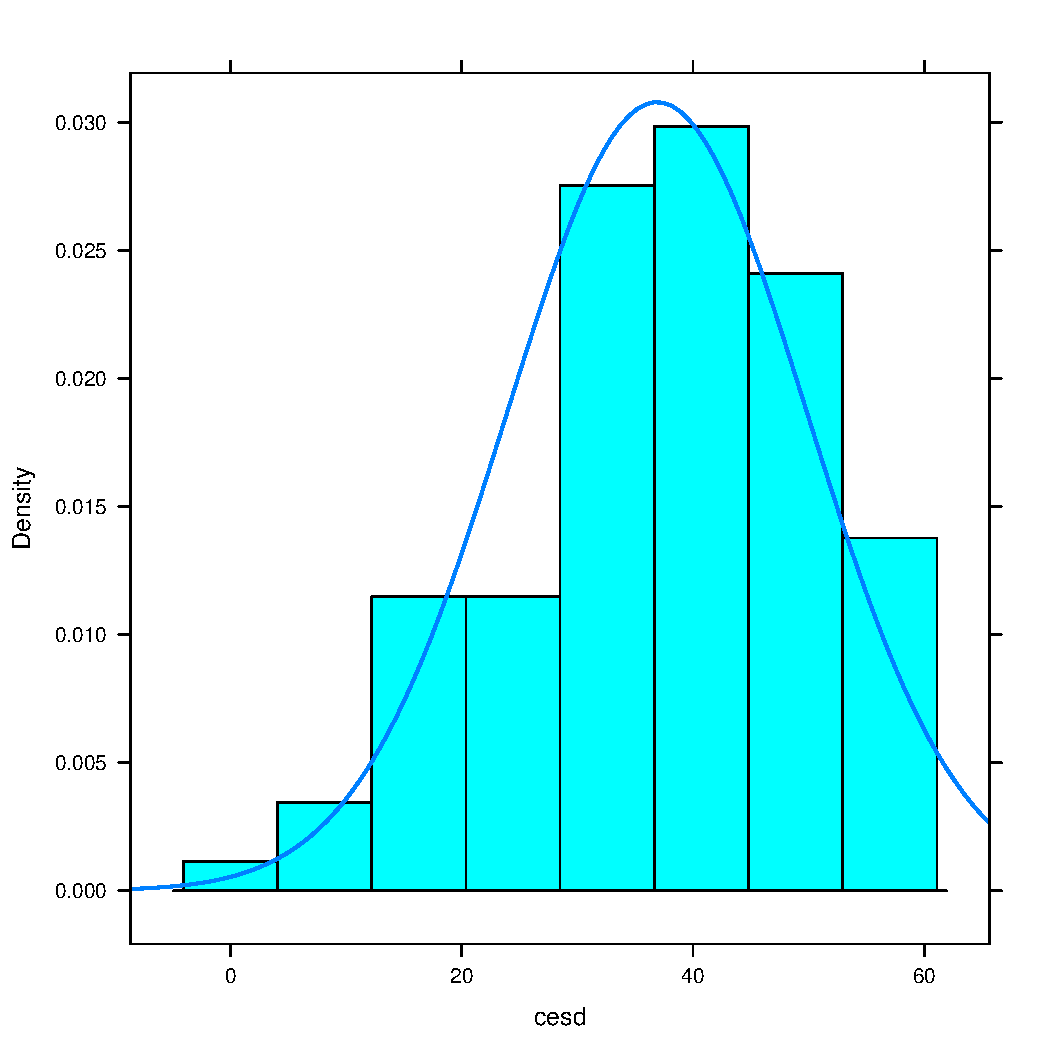
\includegraphics[width=\maxwidth]{figure/women-cesd-hist-1} 

\end{knitrout}

Alternatively, we can make side-by-side plots to compare multiple subsets.
\begin{knitrout}
\definecolor{shadecolor}{rgb}{0.969, 0.969, 0.969}\color{fgcolor}\begin{kframe}
\begin{alltt}
\hlkwd{histogram}\hlstd{(}\hlopt{~} \hlstd{cesd} \hlopt{|} \hlstd{sex,} \hlkwc{data}\hlstd{=HELPrct)}
\end{alltt}
\end{kframe}
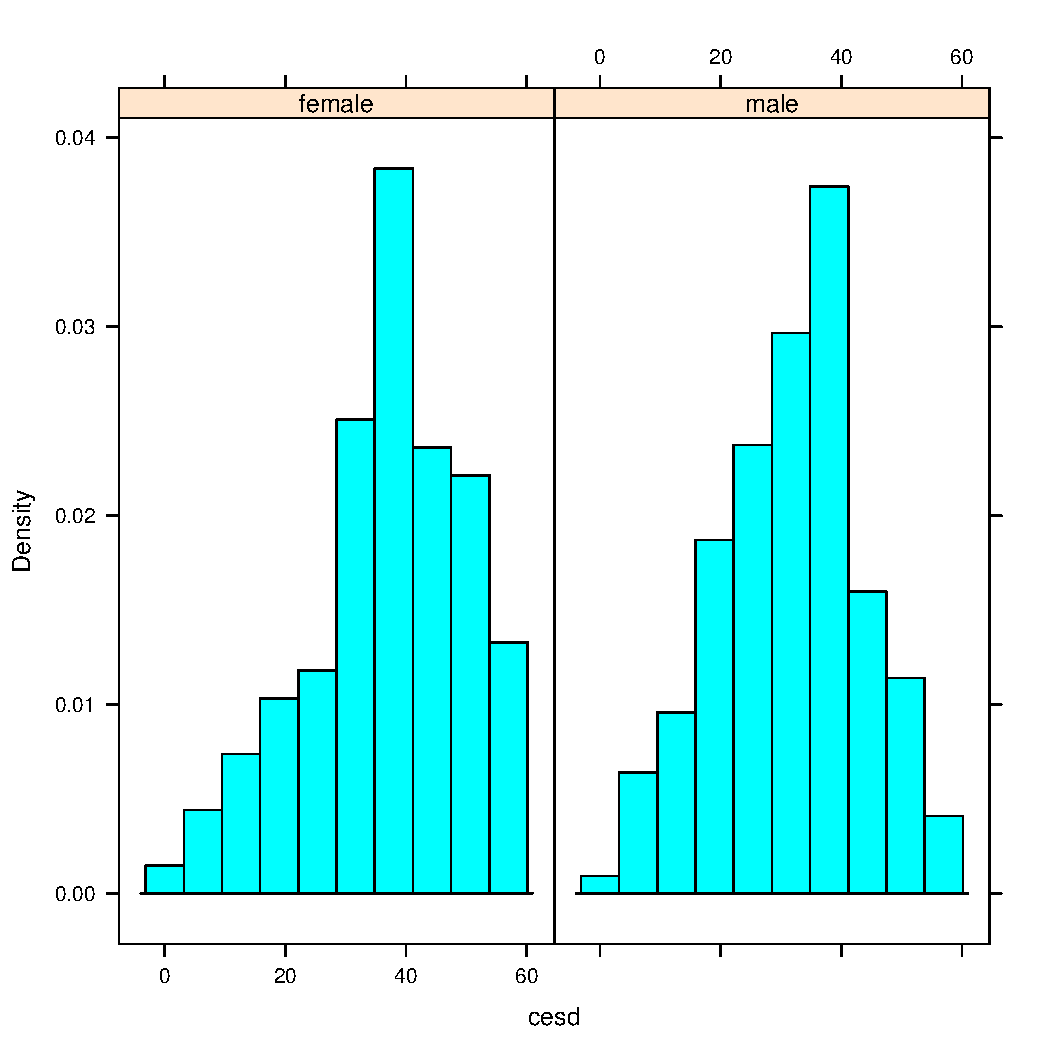
\includegraphics[width=\maxwidth]{figure/cesd-male-female-1} 

\end{knitrout}

The layout can be rearranged.
\Rindex{layout option}%
\begin{center}
\begin{knitrout}
\definecolor{shadecolor}{rgb}{0.969, 0.969, 0.969}\color{fgcolor}\begin{kframe}
\begin{alltt}
\hlkwd{histogram}\hlstd{(}\hlopt{~} \hlstd{cesd} \hlopt{|} \hlstd{sex,} \hlkwc{layout}\hlstd{=}\hlkwd{c}\hlstd{(}\hlnum{1}\hlstd{,} \hlnum{2}\hlstd{),} \hlkwc{data}\hlstd{=HELPrct)}
\end{alltt}
\end{kframe}
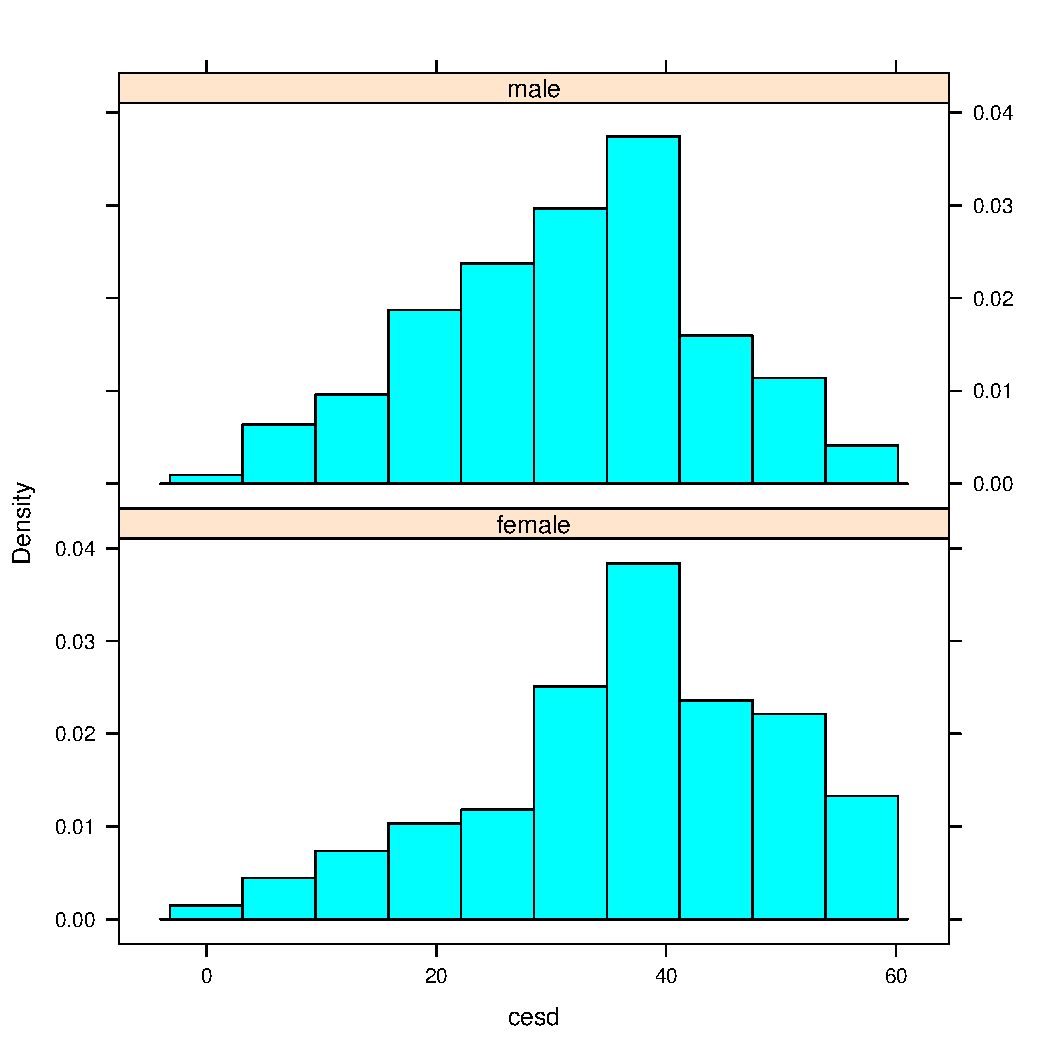
\includegraphics[width=\maxwidth]{figure/cesd-dotlayout-1} 

\end{knitrout}
\end{center}
\begin{problem}
Using the \dataframe{HELPrct} dataset, 
create side-by-side histograms of the CESD scores by substance abuse
group, just for the male subjects, with an overlaid normal density.
\end{problem}%
\begin{solution}
\begin{knitrout}
\definecolor{shadecolor}{rgb}{0.969, 0.969, 0.969}\color{fgcolor}\begin{kframe}
\begin{alltt}
\hlkwd{histogram}\hlstd{(}\hlopt{~} \hlstd{cesd} \hlopt{|} \hlstd{substance,} \hlkwc{fit}\hlstd{=}\hlstr{"normal"}\hlstd{,}
  \hlkwc{data}\hlstd{=}\hlkwd{filter}\hlstd{(HELPrct, sex}\hlopt{==}\hlstr{'male'}\hlstd{))}
\end{alltt}
\end{kframe}
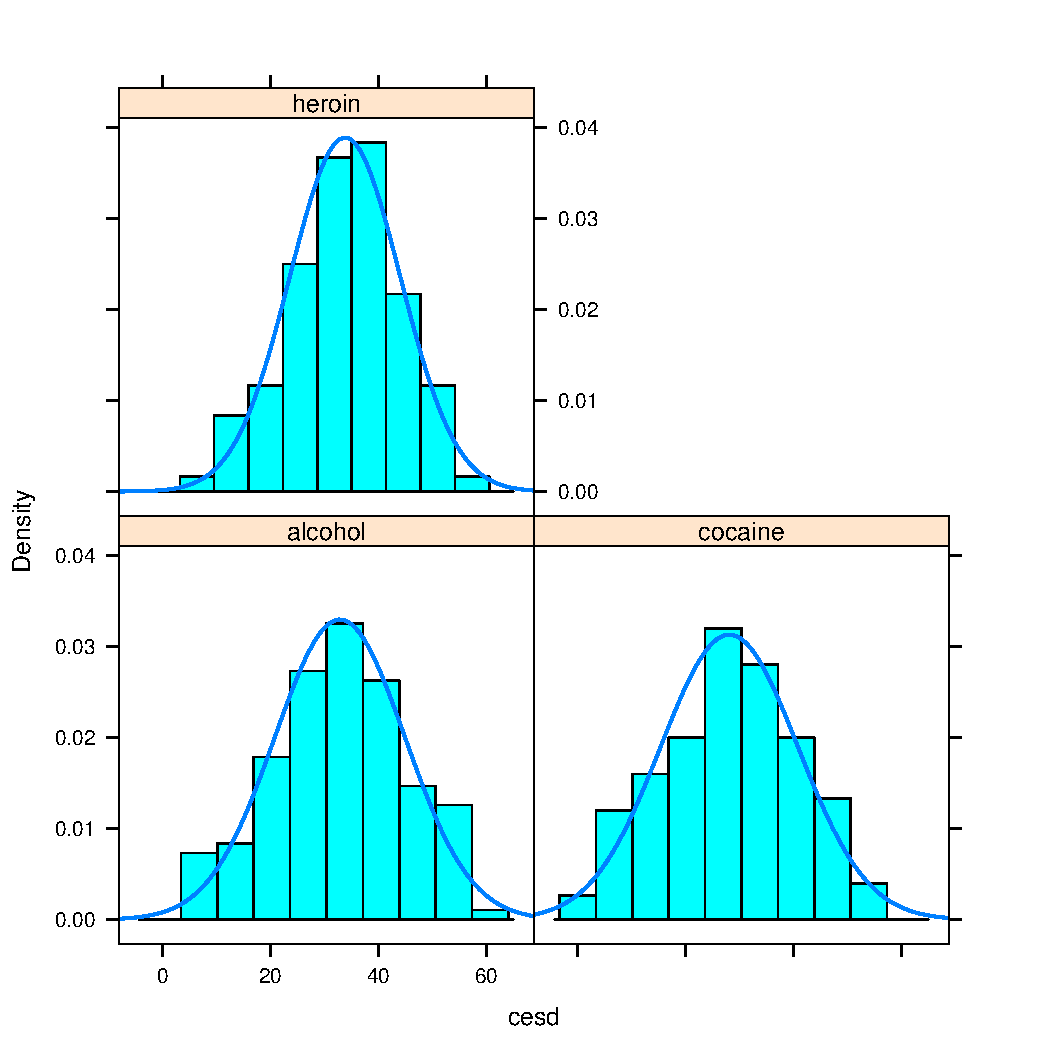
\includegraphics[width=\maxwidth]{figure/subsmale-1} 

\end{knitrout}
\end{solution}%
We can control the number of bins in a number of ways.  These can be specified 
as the total number.
\Rindex{nint option}%
\begin{center}
\begin{knitrout}
\definecolor{shadecolor}{rgb}{0.969, 0.969, 0.969}\color{fgcolor}\begin{kframe}
\begin{alltt}
\hlkwd{histogram}\hlstd{(}\hlopt{~} \hlstd{cesd,} \hlkwc{nint}\hlstd{=}\hlnum{20}\hlstd{,} \hlkwc{data}\hlstd{=female)}
\end{alltt}
\end{kframe}
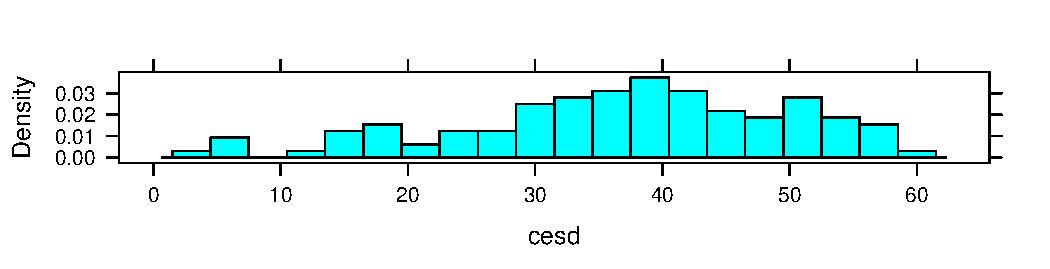
\includegraphics[width=\maxwidth]{figure/cesd-dot-1} 

\end{knitrout}
\end{center}
The width of the bins can be specified.
\Rindex{width option}%
\begin{center}
\begin{knitrout}
\definecolor{shadecolor}{rgb}{0.969, 0.969, 0.969}\color{fgcolor}\begin{kframe}
\begin{alltt}
\hlkwd{histogram}\hlstd{(}\hlopt{~} \hlstd{cesd,} \hlkwc{width}\hlstd{=}\hlnum{2}\hlstd{,} \hlkwc{data}\hlstd{=female)}
\end{alltt}
\end{kframe}
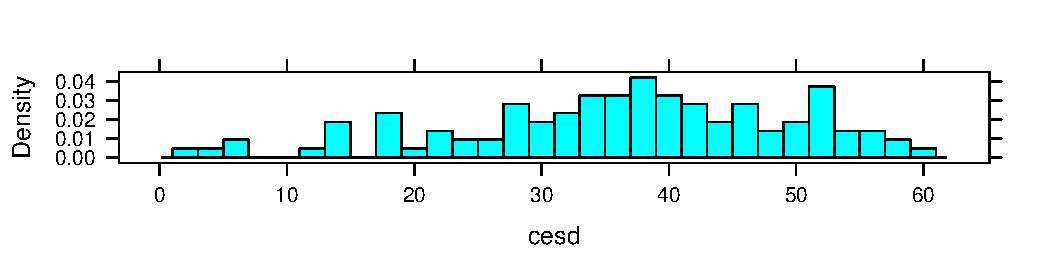
\includegraphics[width=\maxwidth]{figure/cesd-dotwidth-1} 

\end{knitrout}
\end{center}

The \function{dotPlot()} function is used to create a dotplot
for a smaller subset of subjects (homeless females).  We also demonstrate
how to change the x-axis label.
\Rindex{dotPlot()}%
\begin{knitrout}
\definecolor{shadecolor}{rgb}{0.969, 0.969, 0.969}\color{fgcolor}\begin{kframe}
\begin{alltt}
\hlkwd{dotPlot}\hlstd{(}\hlopt{~} \hlstd{cesd,} \hlkwc{xlab}\hlstd{=}\hlstr{"CESD score"}\hlstd{,}
  \hlkwc{data}\hlstd{=}\hlkwd{filter}\hlstd{(HELPrct, (sex}\hlopt{==}\hlstr{"female"}\hlstd{)} \hlopt{&} \hlstd{(homeless}\hlopt{==}\hlstr{"homeless"}\hlstd{)))}
\end{alltt}
\end{kframe}
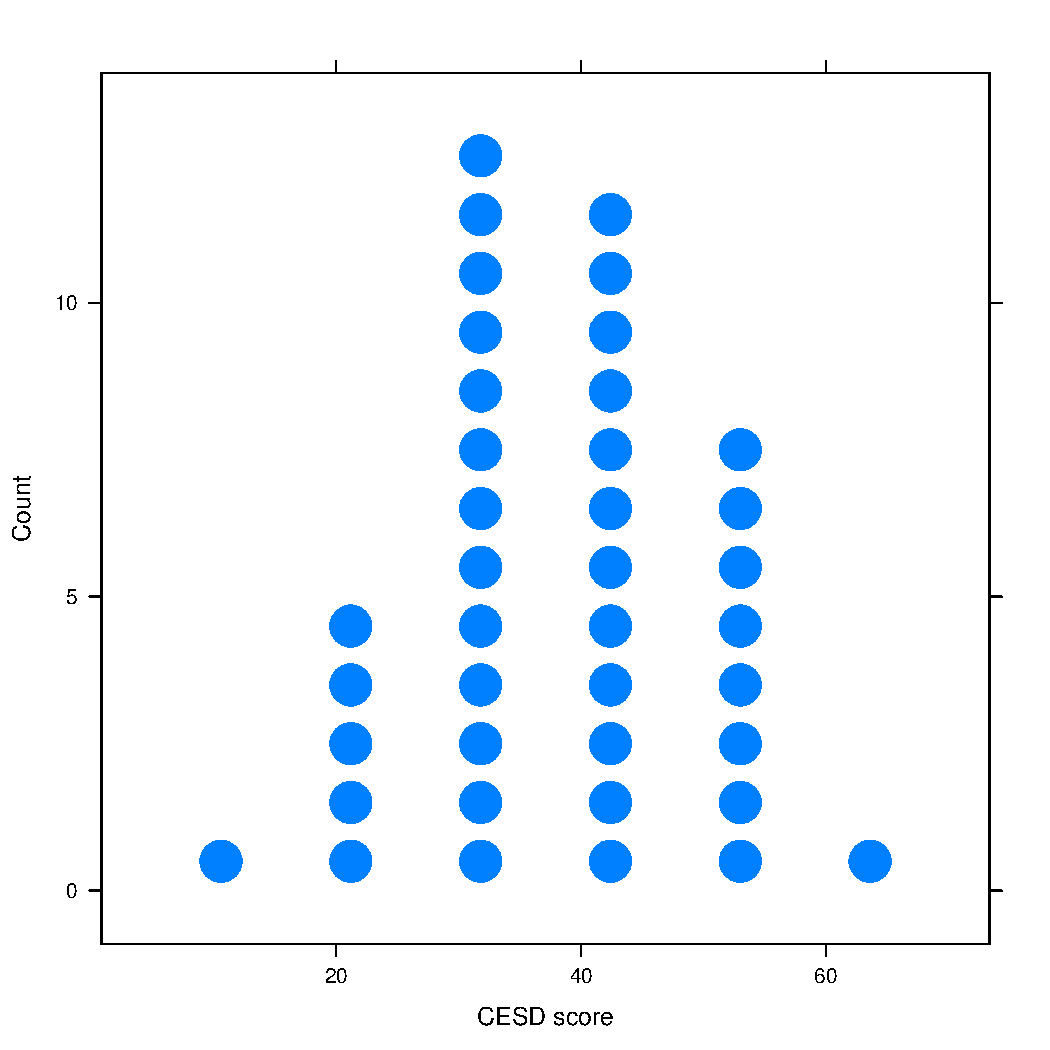
\includegraphics[width=\maxwidth]{figure/cesd-dot4-1} 

\end{knitrout}


\section{Density curves}

\FoodForThought{Density plots are also sensitive to certain choices.  If your density plot is too jagged or too smooth, try changing the \option{adjust} argument: larger than 1 for smoother plots, less than 1 for more jagged plots.} One disadvantage of histograms is that they can be sensitive to the choice of the number of bins.  Another display to consider is a density curve.

Here we adorn a density plot with some additions to demonstrate how to build up a graphic for pedagogical purposes. We add some text, a superimposed normal density as well as a vertical line. A variety of line types and colors can be specified, as well as line widths.

\DiggingDeeper{The \function{plotFun()} function can also be used to annotate plots (see section \ref{sec:plotFun}).}
\begin{center}
\Rindex{densityplot()}%
\Rindex{ladd()}%
\Rindex{panel.mathdensity()}%
\Rindex{panel.abline()}%
\Rindex{col option}%
\Rindex{grid.text()}%
\Rindex{lty option}%
\Rindex{lwd option}%
\begin{knitrout}
\definecolor{shadecolor}{rgb}{0.969, 0.969, 0.969}\color{fgcolor}\begin{kframe}
\begin{alltt}
\hlkwd{densityplot}\hlstd{(}\hlopt{~} \hlstd{cesd,} \hlkwc{data}\hlstd{=female)}
\hlkwd{ladd}\hlstd{(}\hlkwd{grid.text}\hlstd{(}\hlkwc{x}\hlstd{=}\hlnum{0.2}\hlstd{,} \hlkwc{y}\hlstd{=}\hlnum{0.8}\hlstd{,} \hlstr{'only females'}\hlstd{))}
\hlkwd{ladd}\hlstd{(}\hlkwd{panel.mathdensity}\hlstd{(}\hlkwc{args}\hlstd{=}\hlkwd{list}\hlstd{(}\hlkwc{mean}\hlstd{=}\hlkwd{mean}\hlstd{(cesd),}
  \hlkwc{sd}\hlstd{=}\hlkwd{sd}\hlstd{(cesd)),} \hlkwc{col}\hlstd{=}\hlstr{"red"}\hlstd{),} \hlkwc{data}\hlstd{=female)}
\hlkwd{ladd}\hlstd{(}\hlkwd{panel.abline}\hlstd{(}\hlkwc{v}\hlstd{=}\hlnum{60}\hlstd{,} \hlkwc{lty}\hlstd{=}\hlnum{2}\hlstd{,} \hlkwc{lwd}\hlstd{=}\hlnum{2}\hlstd{,} \hlkwc{col}\hlstd{=}\hlstr{"grey"}\hlstd{))}
\end{alltt}
\end{kframe}
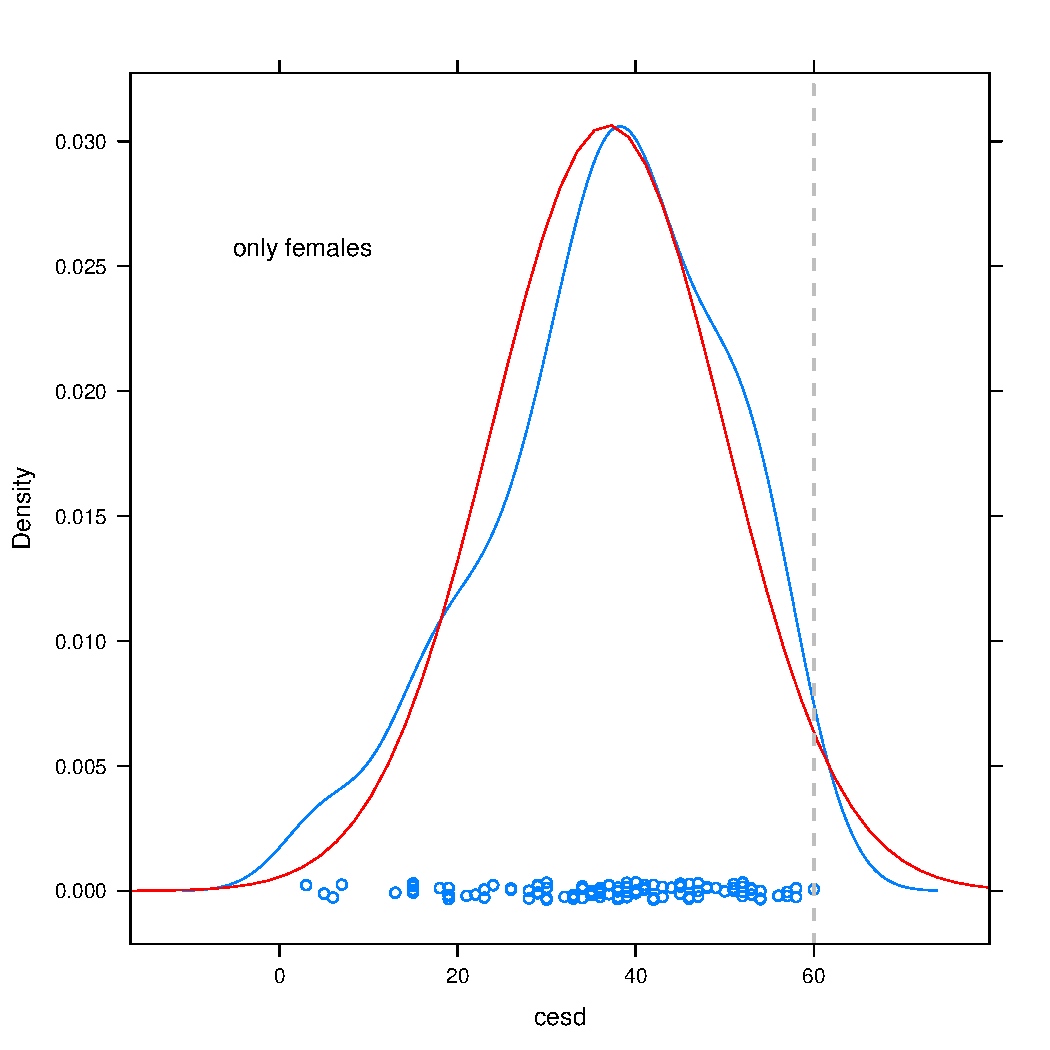
\includegraphics[width=\maxwidth]{figure/dens1-1} 

\end{knitrout}
\end{center}

\section{Frequency polygons}
\myindex{polygons}%

A third option is a frequency polygon, where  the graph is created by joining the midpoints of the top of the bars of a histogram.
\Rindex{freqpolygon()}%
\begin{center}
\begin{knitrout}
\definecolor{shadecolor}{rgb}{0.969, 0.969, 0.969}\color{fgcolor}\begin{kframe}
\begin{alltt}
\hlkwd{freqpolygon}\hlstd{(}\hlopt{~} \hlstd{cesd,} \hlkwc{data}\hlstd{=female)}
\end{alltt}
\end{kframe}
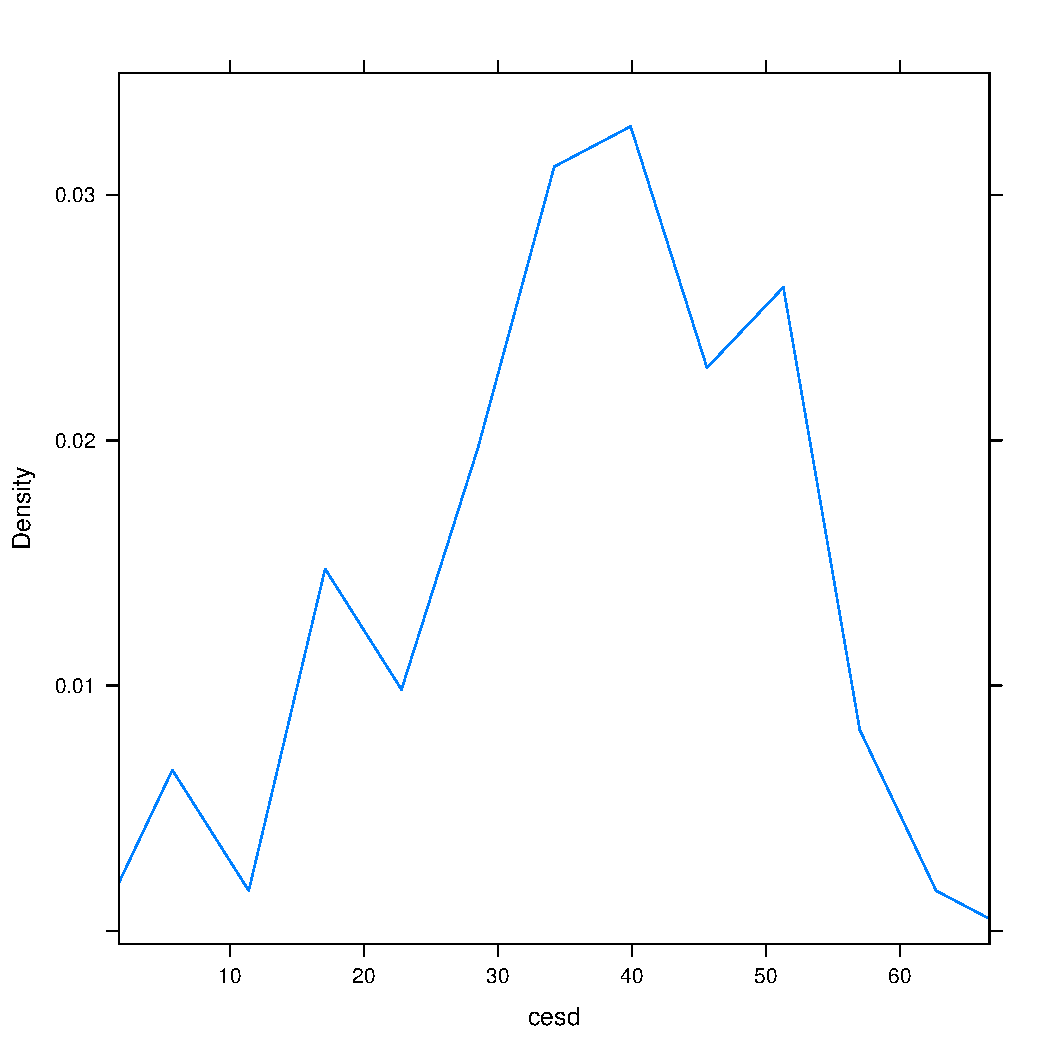
\includegraphics[width=2.5in]{figure/poly-1} 

\end{knitrout}
\end{center}

\section{Normal distributions}

\FoodForThought{\code{x} is for eXtra.}%
The most famous density curve is a normal distribution.  The \function{xpnorm()} function displays the probability that a random variable is less than the first argument, for a normal distribution with mean given by the second argument and standard deviation by the third. More information about probability distributions can be found in section \ref{sec:probability}.

\begin{knitrout}
\definecolor{shadecolor}{rgb}{0.969, 0.969, 0.969}\color{fgcolor}\begin{kframe}
\begin{alltt}
\hlkwd{xpnorm}\hlstd{(}\hlnum{1.96}\hlstd{,} \hlkwc{mean}\hlstd{=}\hlnum{0}\hlstd{,} \hlkwc{sd}\hlstd{=}\hlnum{1}\hlstd{)}
\end{alltt}


{\ttfamily\noindent\itshape\color{messagecolor}{\#\# }}

{\ttfamily\noindent\itshape\color{messagecolor}{\#\# If X \textasciitilde{} N(0, 1), then}}

{\ttfamily\noindent\itshape\color{messagecolor}{\#\# 	P(X <= 1.96) = P(Z <= 1.96) = 0.975}}

{\ttfamily\noindent\itshape\color{messagecolor}{\#\# 	P(X >\ \ 1.96) = P(Z >\ \ 1.96) = 0.025}}

{\ttfamily\noindent\itshape\color{messagecolor}{\#\# }}\end{kframe}
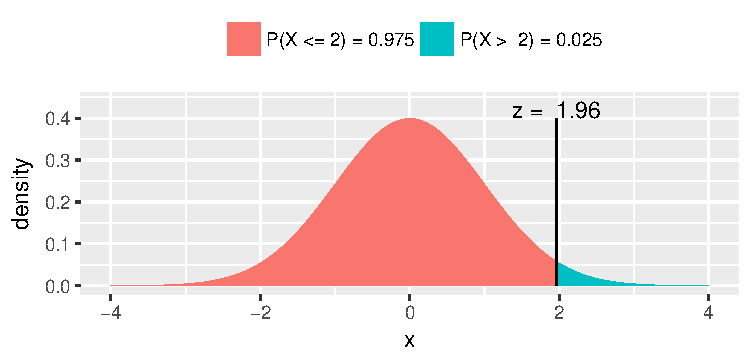
\includegraphics[width=\maxwidth]{figure/norm1-1} 
\begin{kframe}\begin{verbatim}
## [1] 0.975
\end{verbatim}
\end{kframe}
\end{knitrout}


\section{Inference for a single sample}
\label{sec:bootstrapsing}

\Rindex{t.test()}%
\Rindex{confint()}%

We can calculate a 95\% confidence interval for the mean CESD 
score for females by using a t-test:
\begin{knitrout}
\definecolor{shadecolor}{rgb}{0.969, 0.969, 0.969}\color{fgcolor}\begin{kframe}
\begin{alltt}
\hlkwd{t.test}\hlstd{(}\hlopt{~} \hlstd{cesd,} \hlkwc{data}\hlstd{=female)}
\end{alltt}
\begin{verbatim}
## 
## 	One Sample t-test
## 
## data:  cesd
## t = 29, df = 110, p-value <2e-16
## alternative hypothesis: true mean is not equal to 0
## 95 percent confidence interval:
##  34.39 39.38
## sample estimates:
## mean of x 
##     36.89
\end{verbatim}
\begin{alltt}
\hlkwd{confint}\hlstd{(}\hlkwd{t.test}\hlstd{(}\hlopt{~} \hlstd{cesd,} \hlkwc{data}\hlstd{=female))}
\end{alltt}
\begin{verbatim}
##   mean of x lower upper level
## 1     36.89 34.39 39.38  0.95
\end{verbatim}
\end{kframe}
\end{knitrout}

\DiggingDeeper{More details and examples can be found in the 
\pkg{mosaic} package Resampling Vignette.}
\myindex{bootstrapping}%
\myindex{resampling}%
But it's also straightforward to calculate this using a bootstrap.
The statistic that we want to resample is the mean.  
\begin{knitrout}
\definecolor{shadecolor}{rgb}{0.969, 0.969, 0.969}\color{fgcolor}\begin{kframe}
\begin{alltt}
\hlkwd{mean}\hlstd{(}\hlopt{~} \hlstd{cesd,} \hlkwc{data}\hlstd{=female)}
\end{alltt}
\begin{verbatim}
## [1] 36.89
\end{verbatim}
\end{kframe}
\end{knitrout}

One resampling trial can be carried out:
\FoodForThought{Here we sample with replacement from the original dataframe,
creating a resampled dataframe with the same number of rows.}
\Rindex{resample()}%
\begin{knitrout}
\definecolor{shadecolor}{rgb}{0.969, 0.969, 0.969}\color{fgcolor}\begin{kframe}
\begin{alltt}
\hlkwd{mean}\hlstd{(}\hlopt{~} \hlstd{cesd,} \hlkwc{data}\hlstd{=}\hlkwd{resample}\hlstd{(female))}
\end{alltt}
\begin{verbatim}
## [1] 35.36
\end{verbatim}
\end{kframe}
\end{knitrout}
\FoodForThought{Even though a single trial is of little use, it's smart having
students do the calculation to show that they are (usually!) getting a different
result than without resampling.}

Another will yield different results:
\begin{knitrout}
\definecolor{shadecolor}{rgb}{0.969, 0.969, 0.969}\color{fgcolor}\begin{kframe}
\begin{alltt}
\hlkwd{mean}\hlstd{(}\hlopt{~} \hlstd{cesd,} \hlkwc{data}\hlstd{=}\hlkwd{resample}\hlstd{(female))}
\end{alltt}
\begin{verbatim}
## [1] 38.02
\end{verbatim}
\end{kframe}
\end{knitrout}

Now conduct 1000 resampling trials, saving the results in an object
called \texttt{trials}:
\Rindex{do()}%
\Rindex{qdata()}%
\begin{knitrout}
\definecolor{shadecolor}{rgb}{0.969, 0.969, 0.969}\color{fgcolor}\begin{kframe}
\begin{alltt}
\hlstd{trials} \hlkwb{<-} \hlkwd{do}\hlstd{(}\hlnum{1000}\hlstd{)} \hlopt{*} \hlkwd{mean}\hlstd{(}\hlopt{~} \hlstd{cesd,} \hlkwc{data}\hlstd{=}\hlkwd{resample}\hlstd{(female))}
\hlkwd{head}\hlstd{(trials,} \hlnum{3}\hlstd{)}
\end{alltt}
\begin{verbatim}
##    mean
## 1 37.69
## 2 37.07
## 3 38.49
\end{verbatim}
\begin{alltt}
\hlkwd{qdata}\hlstd{(}\hlopt{~} \hlstd{mean,} \hlkwd{c}\hlstd{(}\hlnum{.025}\hlstd{,} \hlnum{.975}\hlstd{),} \hlkwc{data}\hlstd{=trials)}
\end{alltt}
\begin{verbatim}
##       quantile     p
## 2.5%     34.30 0.025
## 97.5%    39.34 0.975
\end{verbatim}
\end{kframe}
\end{knitrout}
